\section{Auswertung}
\label{sec:Auswertung}
In diesem Versuch werden Messdaten aufgenommen und zusammen mit zuvor simulierten Daten analysiert. So lassen sich die gemessenen Größen mit dem Theoriemodell abgleichen.
Die Messdaten werden bei ausgeschaltetem Raumlicht aufgenommen und zu jedem Messwert werden die Dunkelzählraten (Zählraten ohne LED Signal) subtrahiert, um 
ein Maß für die bereinigte Intensität zu erhalten. Jede Messung erfolgt mit einer Integrationszeit von $\qty{10000}{\micro\second}$ und wird fünfmal gemittelt.

\subsection{Spektrometermessung mit- und ohne Raumlicht}
Zuerst wird untersucht, welchen Effekt das Umgebungslicht auf die Auswertung des Versuches hätte. Dazu wird jeweils eine Spektrometermessung mit eingeschaltetem Raumlicht 
und eine Messung ohne Licht durchgeführt. In \autoref{fig:lights_on1} und \autoref{fig:lights_on2} sind die bereinigte und unbereinigte Intensität gegen die Wellenlänge aufgetragen.
\begin{figure}
  \centering
  \begin{subfigure}{0.7\textwidth}
    \includegraphics[width = \textwidth]{lights_on1.pdf}
    \caption{Unbereinigte Intensität}
    \label{fig:lights_on1}
  \end{subfigure}
  \hfill
  \begin{subfigure}{0.7\textwidth}
    \includegraphics[width = \textwidth]{lights_on2.pdf}
    \caption{Bereinigte Intensität}
    \label{fig:lights_on2}
  \end{subfigure}
  \caption{Bereinigte- und unbereinigte Intensität der Lichtreflexe gegen die Wellenlänge für jeweils eine Spektrometermessung mit- und ohne eingeschaltetem Raumlicht.}
  \label{fig:lights_on}
\end{figure}
Wie sich erkennen lässt, liegt die unbereinigte Intensität der Messung mit äußerem Lichteinfluss weit über jener ohne Raumlicht. Dies wirkt sich stark auf die Fluktuation 
der Dunkelzählraten bereinigten Messwerte aus, wie sich unschwer in \autoref{fig:lights_on2} erkennen lässt. Daher sollte immer ohne äußere Lichteinwirkung gemessen werden.

\subsection{Radialsymmetrie}
Für die Winkelverteilung des am Faserende austretenden Lichtes wird eine Radialsymmetrie erwartet. Um dies zu überprüfen wird die Lichtintensität einer Messung unter Variation
der horizontalen- und vertikalen Winkel in einem zweidimensionalem Diagramm aufgetragen.
\begin{figure}
  \centering
  \includegraphics[width = .6\textwidth]{radial.pdf}
  \caption{Gemessene Intensitätsverteilung gegen horizontalen und vertikalen Winkel.}
  \label{fig:radial}
\end{figure}
Wie sich an \autoref{fig:radial} erkennen lässt, folgt die Winkelverteilung tatsächlich einer Radialsymmetrie.

\subsection{Simulationsdaten}
Im nächsten Schritt der Analyse werden die Simulationsdaten vorbereitet. Dazu werden die Dateien der einzelnen Fasern und simulierten Anregungspunkte eingelesen.
Unphysikalische Simulationsfehler, welche einen Austrittsradius größer dem Faserradius vorweisen werden entfernt. Dazu wird ein Schnitt auf die Variable \texttt{r\_exit > 0.125}
angewendet, welche sich über die Austrittspositionen \texttt{y\_exit} und \texttt{z\_exit} berechnen lässt. Die Auswirkung dieser Selektion ist in \autoref{fig:sim_cut} zu sehen.
\begin{figure}
  \centering
  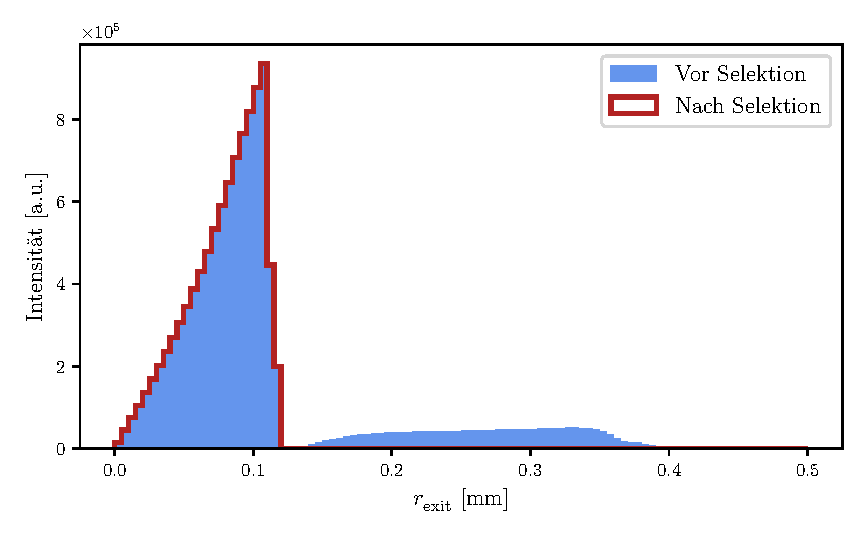
\includegraphics[width = .8\textwidth]{content/pics/r_exit_cut.pdf}
  \caption{Simulationsdaten vor- und nach dem Entfernen unphysikalischer Simulationsfehler.}
  \label{fig:sim_cut}
\end{figure}
Als nächstes werden alle Photonen entfernt, die Rayleigh-Streuungen vollzogen haben. Der Datensatz wird in Kern- und Mantelphotonen (\texttt{length\_clad > 0}) aufgeteilt.
Der Winkel $\Theta$ zur Fasermitte lässt sich anhand des Kosinus des normierten Impulses zur x-Achse bestimmen.
Nach \autoref{!!!Theorie!!!} berechnet sich der maximale Winkel, bei welchem Totalreflexion auftreten kann für die Kern- und Mantelphotonen, die durch die Fasermitte verlaufen zu 
\begin{align*}
  \Theta_\text{max1} &= \symup{arccos}\left(\frac{n_2}{n_1}\right) = \qty{21.37}{\degree} \\
  \Theta_\text{max2} &= \symup{arccos}\left(\frac{n_3}{n_1}\right) = \qty{27.44}{\degree},
\end{align*}
wobei $n_1 \approx \num{1.6}$, $n_2 \approx \num{1.49}$ und $n_3 \approx \num{1.42}$ die Brechungsindices des Kernmaterials und der Mantelmaterialien sind.
Um am Ende der Faser aus dem Material austreten zu können, dürfen die Photonen am Übergang von Faser zu Luft keine Totalreflexion erfahren. 
Die maximalen Winkel zur Faserachse ergeben sich für Photonen im Kern, in der ersten Ummantelung und in der äußeren Ummantelung zu 
\begin{align*}
  \Theta_\text{max3} &= \symup{arcsin}\left(\frac{1}{n_1}\right) = \qty{38.68}{\degree} \\
  \Theta_\text{max4} &= \symup{arccos}\left(\frac{n_2}{n_1}\symup{cos}\left(\symup{arcsin}\left(\frac{1}{n_2}\right)\right)\right) = \qty{46.34}{\degree} \\
  \Theta_\text{max5} &= \symup{arccos}\left(\frac{n_3}{n_1}\symup{cos}\left(\symup{arcsin}\left(\frac{1}{n_3}\right)\right)\right) = \qty{50.94}{\degree}, \\
\end{align*}
respektive. Dabei wird $n \approx 1$ für Luft verwendet.
In \autoref{fig:theta_sim} ist die Winkelverteilung der Kern- und Mantelphotonen histogrammiert. Die theoretisch zu erwartenden, maximalen Winkel sind markiert.
\begin{figure}
  \centering
  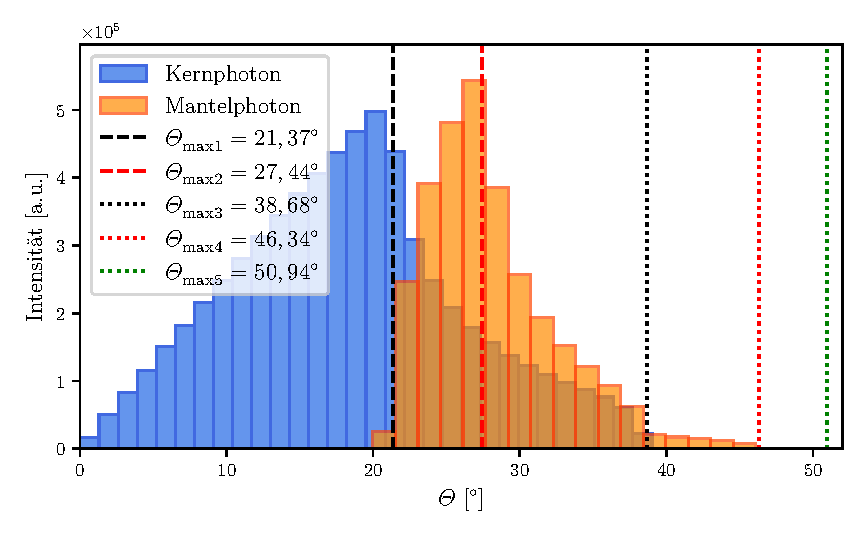
\includegraphics[width = .8\textwidth]{content/pics/theta_sim.pdf}
  \caption{Winkelverteilung der Kern- und Mantelphotonen in den Simulationsdaten. Die Winkel $\Theta_\text{max}$ beschreiben die theoretischen Grenzwinkel der Totalreflexion.}
  \label{fig:theta_sim}
\end{figure}
Die maximalen Winkel der Simulationsdaten lauten 
\begin{align*}
  \Theta_\text{max, Kern} = \qty{39.02}{\degree} \\
  \Theta_\text{max, Mantel} = \qty{46.10}{\degree}.
\end{align*}

Im nächsten Schritt, wird der minimale Abstand \texttt{r\_min} der Photonen zur Fasermitte (Abstand Gerade-Gerade) bestimmt.
In \autoref{fig:rmin_sim} ist die Intensitätsverteilung in einem zweidimensionalem Histogramm gegen den Winkel $\Theta$ und den minimalen Abstand zur Fasermitte \texttt{r\_min},
jeweils für Kern- und Mantelphotonen aufgetragen.
\begin{figure}
  \centering
  \begin{subfigure}{0.45\textwidth}
    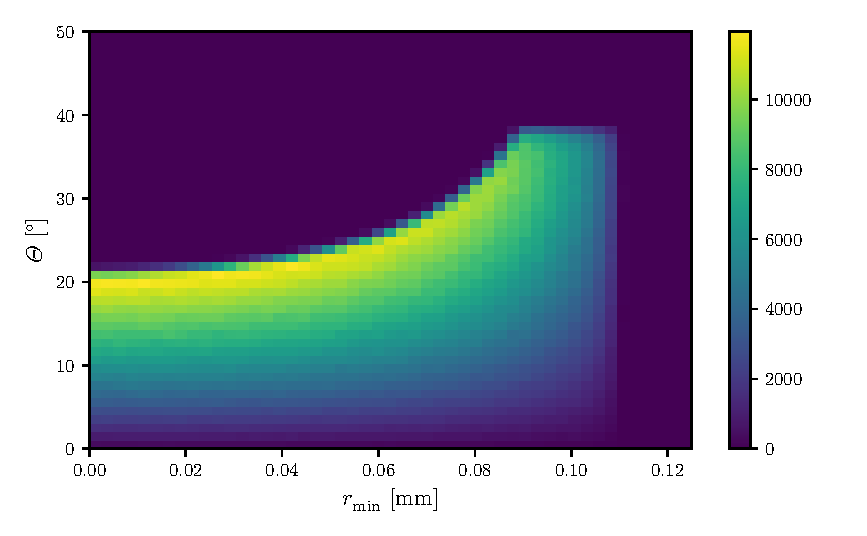
\includegraphics[width = 1.2\textwidth]{content/pics/rmin_sim_core.pdf}
    \caption{Kernphotonen}
    \label{fig:rmin_sim_core}
  \end{subfigure}
  \hfill
  \begin{subfigure}{0.45\textwidth}
    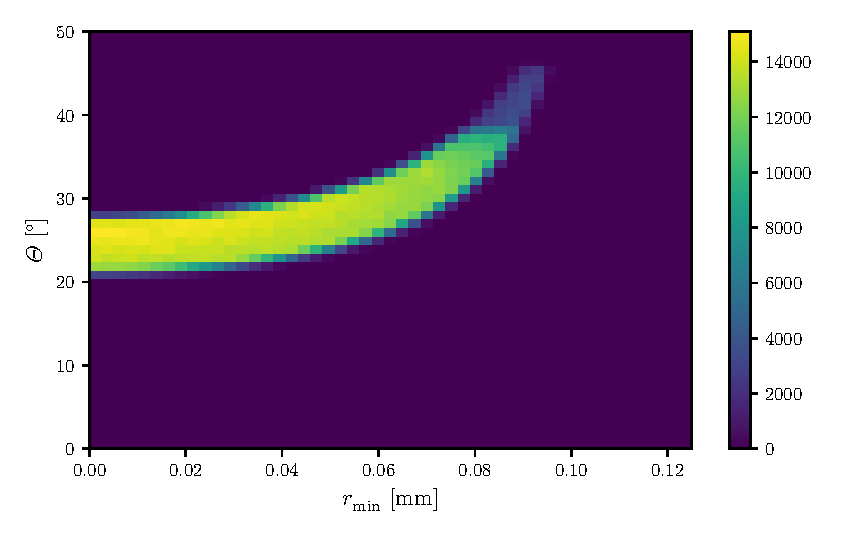
\includegraphics[width = 1.2\textwidth]{content/pics/rmin_sim_cladding.pdf}
    \caption{Mantelphotonen}
    \label{fig:rmin_sim_cladding}
  \end{subfigure}
  \caption{Zweidimensionales Histogramm der Intensitätsverteilung gegen den Winkel $\Theta$ zur Faserachse und den minimalen Abstand zur Fasermitte $r_\text{min}$ für Kern-
  Mantelphotonen.}
  \label{fig:rmin_sim}
\end{figure}
Wie sich erkennen lässt, steigt der maximal erreichte Winkel zur Faserachse mit dem Abstand zu dieser an, was der Erwartung entspricht.
Das Band der Kernphotonen endet für \texttt{r\_min = 0} ungefähr, bei dem Maximalwinkel der Totalreflexion an der ersten Faserummantellung ($\Theta_1$). Das Band der 
Mantelphotonen beginnt dort und endet bei dem Maximalwinkel der Totalreflexion an der Faserhülle ($\Theta_2$), was ebenfalls den Erwartungen entspricht.

\subsection{Absorptionsverhalten}
Als nächstes wird das Absorptionsverhalten der Photonen in der Faser untersucht.  
Dazu wird zu jedem gemessenen Winkel der Intensitätsmessung die Abschwächung der Intensität abhängig vom Anregungsort betrachtet. Mittels \textit{scipy} \cite{scipy}
wird eine exponentielle Funktion der Form $I(x) = I_0 \mathrm{e}^{-ax}$ an die Messdaten gefittet. Dieses Vorgehen ist in \autoref{fig:fits_absorption} für die 10 gemessenen Winkel 
dargestellt.
\begin{figure}
  \centering
  \includegraphics[width = .7\textwidth]{fits_absorption.pdf}
  \caption{Fits zur Bestimmung des Absorptionskoeffizienten für die vermessenen Winkel. Die exponentiellen Fits sind mit einer gestrichelten Linie eingezeichnet.}
  \label{fig:fits_absorption}
\end{figure}
Es ergibt sich ein Durschnittswert des Absorptionskoeffizienten von $a_\text{avg, exp} = \qty{2.1653e-4}{\per\milli\metre}$.
Ein analoges Verfahren wird auf die Simulationsdaten angewendet, wobei hier die Winkel kontinuierlich verlaufen und deshalb in 100 Bins unterteilt werden. 
Hier ergibt sich ein Mittelwert von  $a_\text{avg, theo} = \qty{1.9571e-4}{\per\milli\metre}$.
Die Winkelabhängigkeit des Absorptionskoeffizienten kann \autoref{fig:absorptioncoefficient} entnommen werden. Die jeweiligen Fitparameter werden dabei gegen den Winkel aufgetragen.
Ebenfalls ist die Theoriekurve des winkelabhängigen Absorptionskoeffizienten nach \autoref{!!!!Theorie!!!} eingezeichnet.
\begin{figure}
  \centering
  \begin{subfigure}{.7\textwidth}
    \includegraphics[width = \textwidth]{absorption_coefficient.pdf}
    \caption{Messdaten}
    \label{fig:absorptioncoefficient_data}
  \end{subfigure}
  \hfill
  \begin{subfigure}{.7\textwidth}
    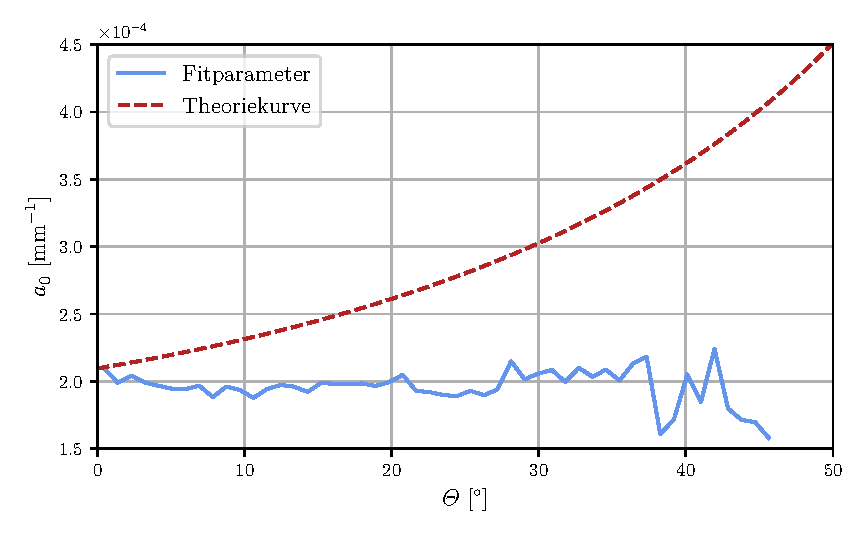
\includegraphics[width = \textwidth]{content/pics/absorption_sim2.pdf}
    \caption{Simulationsdaten}
    \label{fig:absorptioncoefficient_sim}
  \end{subfigure}
  \caption{Winkelabhängigkeit des Absorptionskoeffizienten für die Mess- und Simulationsdaten.}
  \label{fig:absorptioncoefficient}
\end{figure}

\subsection{Winkelintensitätsmessung}
Zuletzt wird der Winkel maximaler Intensität mithilfe einer feinschrittigen Winkelintensitätsmessung bestimmt. 
Dazu könnne die in \autoref{fig:intensity_angle} dargestellten Daten verwendet werden. Aus der Abbildung kann der Winkel maximaler Intensität 
als $\Theta = \qty{11}{\degree}$ entnommen werden.
\begin{figure}
  \centering
  \includegraphics[width = .7\textwidth]{intensity_angle.pdf}
  \caption{Intensitätsverteilung der Messdaten gegen den horizontalen Winkel.}
  \label{fig:intensity_angle}
\end{figure}
